\section{XMToggle\-Button  Class Reference}
\label{classXMToggleButton}\index{XMToggleButton@{XMToggle\-Button}}
{\tt \#include $<$XMPushbutton.h$>$}

Inheritance diagram for XMToggle\-Button::\begin{figure}[H]
\begin{center}
\leavevmode
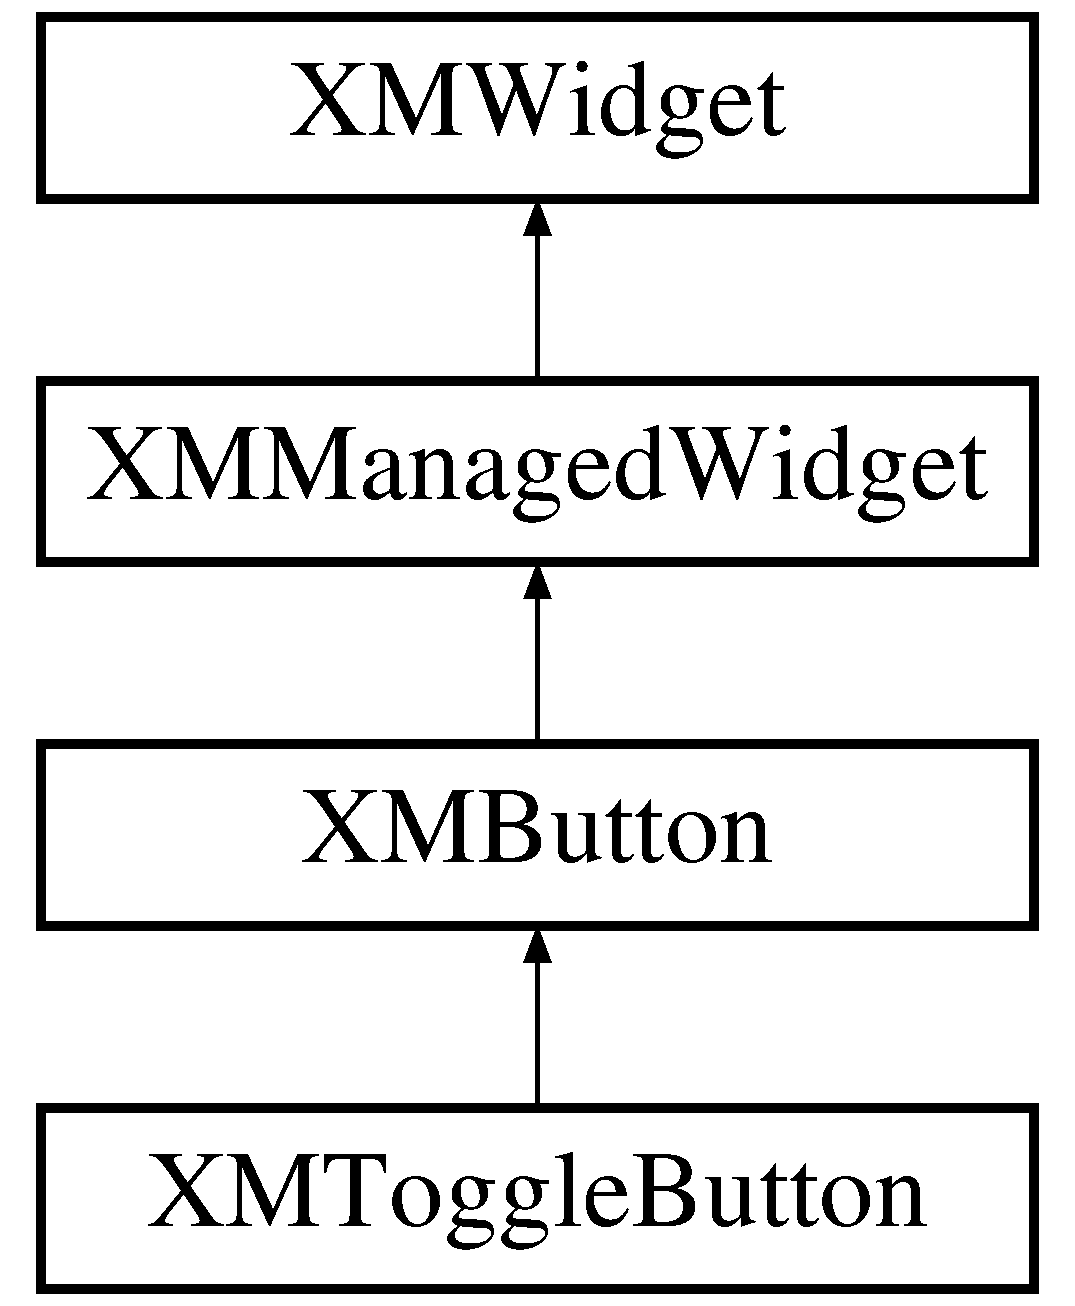
\includegraphics[height=4cm]{classXMToggleButton}
\end{center}
\end{figure}
\subsection*{Public Methods}
\begin{CompactItemize}
\item 
{\bf XMToggle\-Button} (char $\ast$n, Widget parent, void($\ast$cb)({\bf XMWidget} $\ast$, Xt\-Pointer, Xt\-Pointer)=NULL, Xt\-Pointer cd=NULL)
\item 
{\bf XMToggle\-Button} (char $\ast$n, {\bf XMWidget} \&parent, void($\ast$cb)({\bf XMWidget} $\ast$, Xt\-Pointer, Xt\-Pointer)=NULL, Xt\-Pointer cd=NULL)
\item 
{\bf XMToggle\-Button} (Widget w)
\item 
{\bf Callback\_\-data} $\ast$ {\bf Add\-Callback} (void($\ast$cb)({\bf XMWidget} $\ast$, Xt\-Pointer, Xt\-Pointer)=NULL, Xt\-Pointer cd=NULL)
\item 
void {\bf Show\-Indicator} ()
\item 
void {\bf Hide\-Indicator} ()
\item 
void {\bf Diamond} ()
\item 
void {\bf Box} ()
\item 
void {\bf Set\-State} (Boolean state)
\item 
void {\bf Set} ()
\item 
void {\bf Un\-Set} ()
\item 
Boolean {\bf Get\-State} ()
\end{CompactItemize}


\subsection{Constructor \& Destructor Documentation}
\index{XMToggleButton@{XMToggle\-Button}!XMToggleButton@{XMToggleButton}}
\index{XMToggleButton@{XMToggleButton}!XMToggleButton@{XMToggle\-Button}}
\subsubsection{\setlength{\rightskip}{0pt plus 5cm}XMToggle\-Button::XMToggle\-Button (char $\ast$ {\em n}, Widget {\em parent}, void($\ast$ {\em cb})({\bf XMWidget} $\ast$, Xt\-Pointer, Xt\-Pointer) = NULL, Xt\-Pointer {\em cd} = NULL)\hspace{0.3cm}{\tt  [inline]}}\label{classXMToggleButton_a0}




Definition at line 471 of file XMPushbutton.h.

References XMWidget::Add\-Callback(), and XMButton::Enable().\index{XMToggleButton@{XMToggle\-Button}!XMToggleButton@{XMToggleButton}}
\index{XMToggleButton@{XMToggleButton}!XMToggleButton@{XMToggle\-Button}}
\subsubsection{\setlength{\rightskip}{0pt plus 5cm}XMToggle\-Button::XMToggle\-Button (char $\ast$ {\em n}, {\bf XMWidget} \& {\em parent}, void($\ast$ {\em cb})({\bf XMWidget} $\ast$, Xt\-Pointer, Xt\-Pointer) = NULL, Xt\-Pointer {\em cd} = NULL)\hspace{0.3cm}{\tt  [inline]}}\label{classXMToggleButton_a1}




Definition at line 481 of file XMPushbutton.h.

References XMWidget::Add\-Callback(), and XMButton::Enable().\index{XMToggleButton@{XMToggle\-Button}!XMToggleButton@{XMToggleButton}}
\index{XMToggleButton@{XMToggleButton}!XMToggleButton@{XMToggle\-Button}}
\subsubsection{\setlength{\rightskip}{0pt plus 5cm}XMToggle\-Button::XMToggle\-Button (Widget {\em w})\hspace{0.3cm}{\tt  [inline]}}\label{classXMToggleButton_a2}




Definition at line 490 of file XMPushbutton.h.

\subsection{Member Function Documentation}
\index{XMToggleButton@{XMToggle\-Button}!AddCallback@{AddCallback}}
\index{AddCallback@{AddCallback}!XMToggleButton@{XMToggle\-Button}}
\subsubsection{\setlength{\rightskip}{0pt plus 5cm}{\bf Callback\_\-data}$\ast$ XMToggle\-Button::Add\-Callback (void($\ast$ {\em cb})({\bf XMWidget} $\ast$, Xt\-Pointer, Xt\-Pointer) = NULL, Xt\-Pointer {\em cd} = NULL)\hspace{0.3cm}{\tt  [inline]}}\label{classXMToggleButton_a3}




Definition at line 497 of file XMPushbutton.h.

References XMWidget::Add\-Callback().\index{XMToggleButton@{XMToggle\-Button}!Box@{Box}}
\index{Box@{Box}!XMToggleButton@{XMToggle\-Button}}
\subsubsection{\setlength{\rightskip}{0pt plus 5cm}void XMToggle\-Button::Box ()\hspace{0.3cm}{\tt  [inline]}}\label{classXMToggleButton_a7}




Definition at line 511 of file XMPushbutton.h.

References XMWidget::Set\-Attribute().\index{XMToggleButton@{XMToggle\-Button}!Diamond@{Diamond}}
\index{Diamond@{Diamond}!XMToggleButton@{XMToggle\-Button}}
\subsubsection{\setlength{\rightskip}{0pt plus 5cm}void XMToggle\-Button::Diamond ()\hspace{0.3cm}{\tt  [inline]}}\label{classXMToggleButton_a6}




Definition at line 508 of file XMPushbutton.h.

References XMWidget::Set\-Attribute().\index{XMToggleButton@{XMToggle\-Button}!GetState@{GetState}}
\index{GetState@{GetState}!XMToggleButton@{XMToggle\-Button}}
\subsubsection{\setlength{\rightskip}{0pt plus 5cm}Boolean XMToggle\-Button::Get\-State ()\hspace{0.3cm}{\tt  [inline]}}\label{classXMToggleButton_a11}




Definition at line 521 of file XMPushbutton.h.

References XMWidget::Get\-Attribute().\index{XMToggleButton@{XMToggle\-Button}!HideIndicator@{HideIndicator}}
\index{HideIndicator@{HideIndicator}!XMToggleButton@{XMToggle\-Button}}
\subsubsection{\setlength{\rightskip}{0pt plus 5cm}void XMToggle\-Button::Hide\-Indicator ()\hspace{0.3cm}{\tt  [inline]}}\label{classXMToggleButton_a5}




Definition at line 506 of file XMPushbutton.h.

References XMWidget::Set\-Attribute().\index{XMToggleButton@{XMToggle\-Button}!Set@{Set}}
\index{Set@{Set}!XMToggleButton@{XMToggle\-Button}}
\subsubsection{\setlength{\rightskip}{0pt plus 5cm}void XMToggle\-Button::Set ()\hspace{0.3cm}{\tt  [inline]}}\label{classXMToggleButton_a9}




Definition at line 517 of file XMPushbutton.h.

References XMWidget::Set\-Attribute().\index{XMToggleButton@{XMToggle\-Button}!SetState@{SetState}}
\index{SetState@{SetState}!XMToggleButton@{XMToggle\-Button}}
\subsubsection{\setlength{\rightskip}{0pt plus 5cm}void XMToggle\-Button::Set\-State (Boolean {\em state})\hspace{0.3cm}{\tt  [inline]}}\label{classXMToggleButton_a8}




Definition at line 515 of file XMPushbutton.h.

References XMWidget::Set\-Attribute().\index{XMToggleButton@{XMToggle\-Button}!ShowIndicator@{ShowIndicator}}
\index{ShowIndicator@{ShowIndicator}!XMToggleButton@{XMToggle\-Button}}
\subsubsection{\setlength{\rightskip}{0pt plus 5cm}void XMToggle\-Button::Show\-Indicator ()\hspace{0.3cm}{\tt  [inline]}}\label{classXMToggleButton_a4}




Definition at line 504 of file XMPushbutton.h.

References XMWidget::Set\-Attribute().\index{XMToggleButton@{XMToggle\-Button}!UnSet@{UnSet}}
\index{UnSet@{UnSet}!XMToggleButton@{XMToggle\-Button}}
\subsubsection{\setlength{\rightskip}{0pt plus 5cm}void XMToggle\-Button::Un\-Set ()\hspace{0.3cm}{\tt  [inline]}}\label{classXMToggleButton_a10}




Definition at line 519 of file XMPushbutton.h.

References XMWidget::Set\-Attribute().

The documentation for this class was generated from the following file:\begin{CompactItemize}
\item 
{\bf XMPushbutton.h}\end{CompactItemize}
